\section{Alvan Alvanzah (1174077)}
\subsection{Instalasi Map Server}
\begin{enumerate}
	\item  Download installer Map Server di https://ms4w.com. Pilih yang .exe.
	\hfill\break
	\begin{figure}[H]
		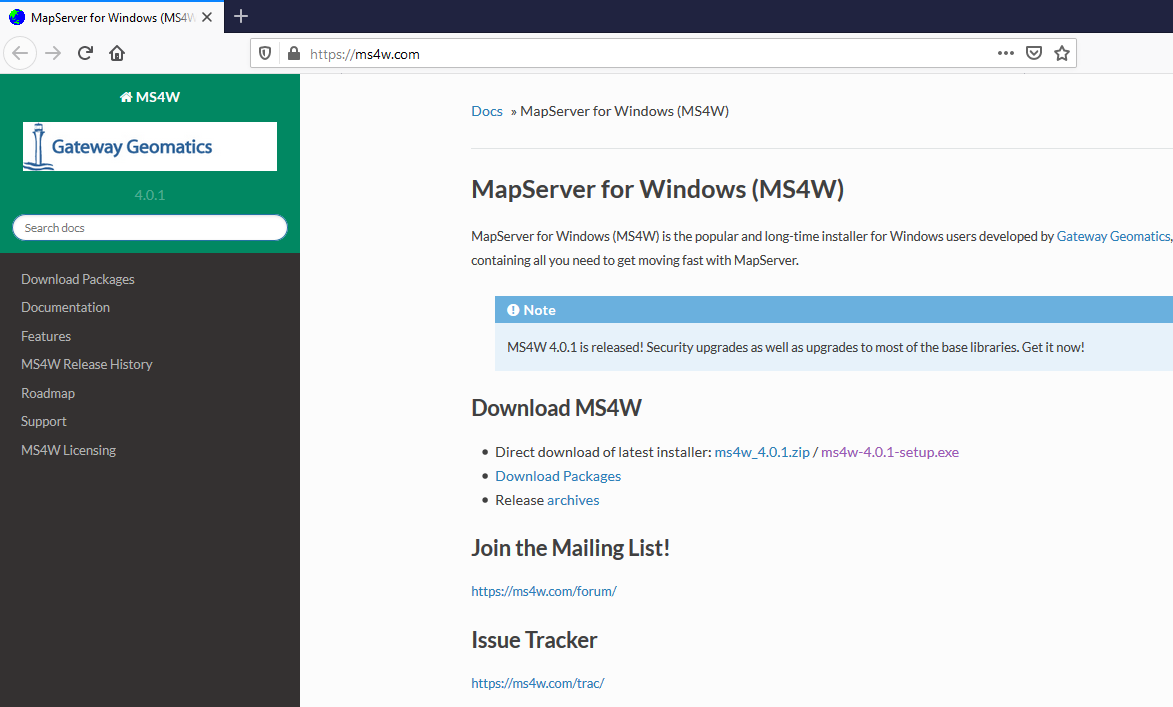
\includegraphics[width=8cm]{figures/Tugas4/1174077/1.png}
		\centering
		\caption{Download installer Map Server.}
	\end{figure}
	\item  Setelah selesai di download, klik dua kali pada installer.
	\hfill\break
	\begin{figure}[H]
		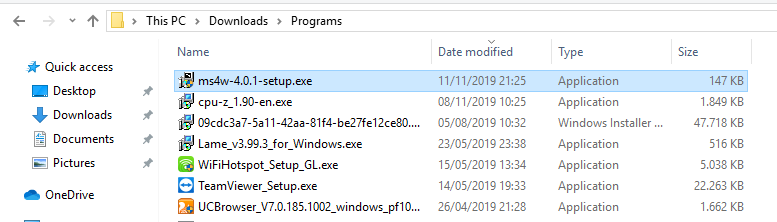
\includegraphics[width=8cm]{figures/Tugas4/1174077/2.png}
		\centering
		\caption{Klik dua kali pada installer.}
	\end{figure}
	\item  Kemudian klik "I Agree".
	\hfill\break
	\begin{figure}[H]
		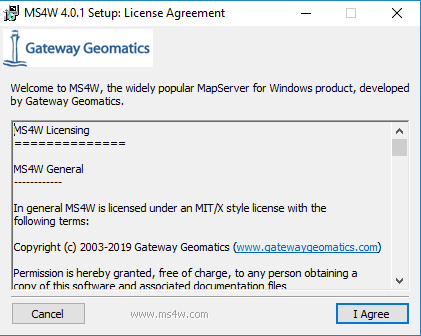
\includegraphics[width=8cm]{figures/Tugas4/1174077/3.png}
		\centering
		\caption{Klik "I Agree".}
	\end{figure}
	\item  Pilih tipe instalasinya yang "Full". Kemudian klik Next.
	\hfill\break
	\begin{figure}[H]
		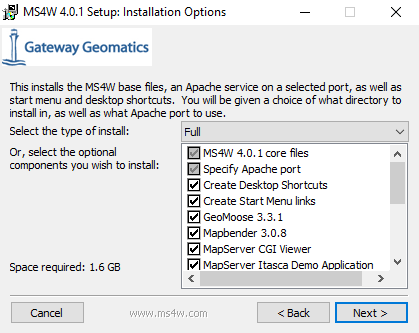
\includegraphics[width=8cm]{figures/Tugas4/1174077/4.png}
		\centering
		\caption{Tipe instalasi "Full".}
	\end{figure}
	\item  Pilih direktori instalasinya. Kemudian klik Next.
	\hfill\break
	\begin{figure}[H]
		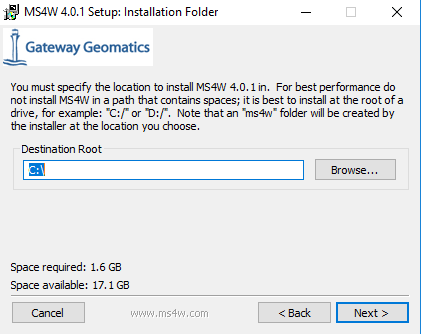
\includegraphics[width=8cm]{figures/Tugas4/1174077/5.png}
		\centering
		\caption{Pilih direktori instalasi}
	\end{figure}
	\item  Isi port Apache yang akan dipakai. Kemudian klik Next.
	\hfill\break
	\begin{figure}[H]
		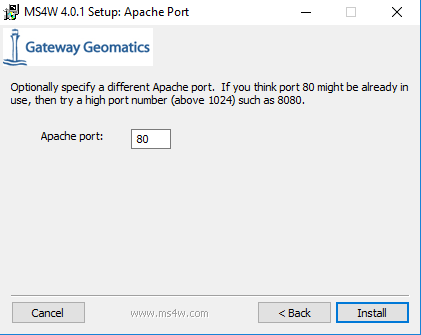
\includegraphics[width=8cm]{figures/Tugas4/1174077/6.png}
		\centering
		\caption{Isi port Apache.}
	\end{figure}
	\item  Tunggu hingga proses instalasi selesai.
	\hfill\break
	\begin{figure}[H]
		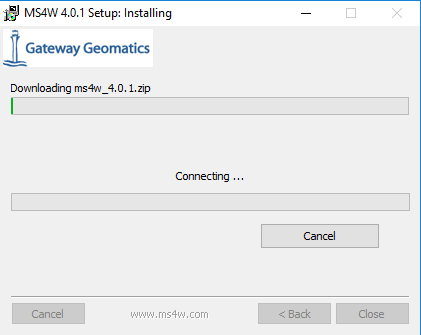
\includegraphics[width=8cm]{figures/Tugas4/1174077/7.png}
		\centering
		\caption{Proses instalasi.}
	\end{figure}
	\item  Klik Close.
	\hfill\break
	\begin{figure}[H]
		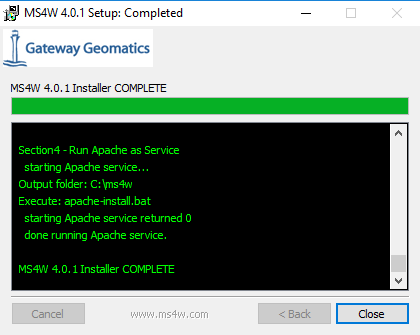
\includegraphics[width=8cm]{figures/Tugas4/1174077/8.png}
		\centering
		\caption{Akhir proses instalasi.}
	\end{figure}
\end{enumerate}
\subsection{Instalasi Map Proxy}
\begin{enumerate}
	\item  Ketik peritah berikut di CMD.
	\hfill\break
	\begin{figure}[H]
		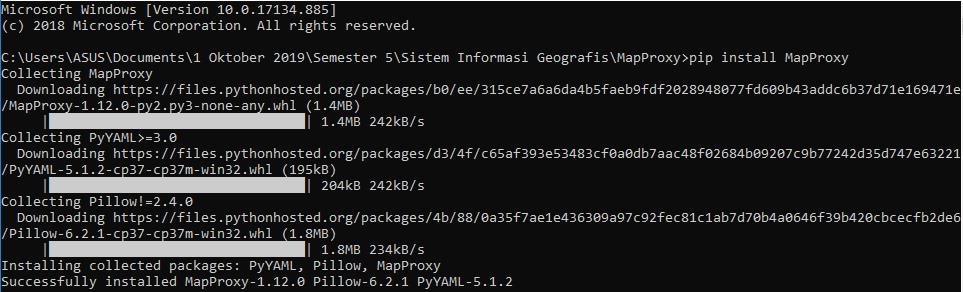
\includegraphics[width=8cm]{figures/Tugas4/1174077/9.png}
		\centering
		\caption{Install Map Proxy}
	\end{figure}
	\item  Ketik peritah berikut di CMD.
	\hfill\break
	\begin{figure}[H]
		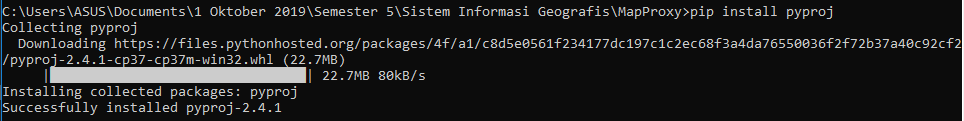
\includegraphics[width=8cm]{figures/Tugas4/1174077/10.png}
		\centering
		\caption{Install pyproj}
	\end{figure}
\end{enumerate}
\subsection{Link Youtube}
https://youtu.be/KEsj1L7oE4c
\subsection{Pengujian}
\begin{enumerate}
  \item Masuk Ke folder httpd.d yang ada di folder ms4w
  \hfill\break
    \begin{figure}[H]
		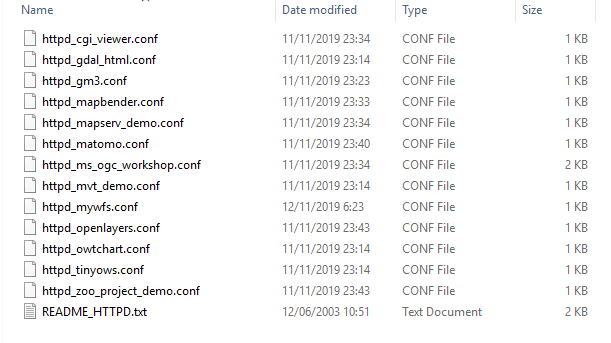
\includegraphics[width=4cm]{figures/Tugas4/1174077/11.png}
		\centering
		\caption{Isi Folder httpd.d}
    \end{figure}
  \item Buat sebuah file dengan nama httpd mywfs conf
  \hfill\break
    \begin{figure}[H]
		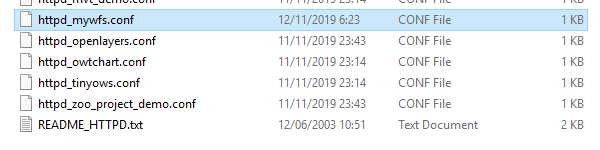
\includegraphics[width=4cm]{figures/Tugas4/1174077/12.png}
		\centering
		\caption{Membuat file baru}
    \end{figure}
  \item Buka file httpd mywfs conf yang baru dibuat dan ubah isinya menjadi seperti berikut
  \hfill\break
    \begin{figure}[H]
		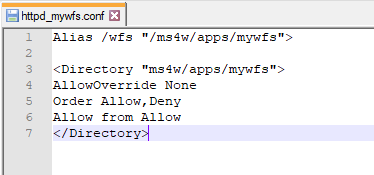
\includegraphics[width=4cm]{figures/Tugas4/1174077/13.png}
		\centering
		\caption{Konfigurasi File Tersebut}
    \end{figure}
  \item Buka Folder apps yang ada di folder ms4w
  \hfill\break
    \begin{figure}[H]
		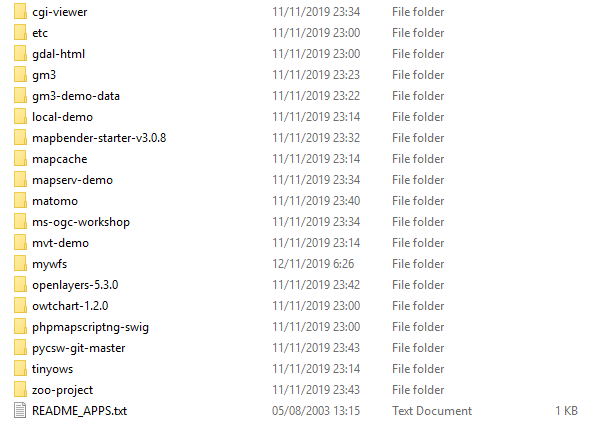
\includegraphics[width=4cm]{figures/Tugas4/1174077/14.png}
		\centering
		\caption{Isi Folder Apps}
    \end{figure}
  \item Buat sebuah folder baru disana dengan nama mywfs,karena sebelumnya menyeting di httpd mywfs conf nya seperti itu
  \hfill\break
    \begin{figure}[H]
		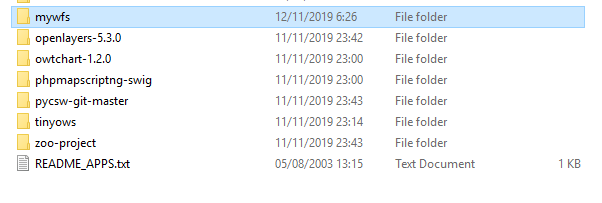
\includegraphics[width=4cm]{figures/Tugas4/1174077/15.png}
		\centering
		\caption{Membuat folder baru}
    \end{figure}
  \item Di dalam folder mywfs buat file baru dengan nama mywfs.map
  \hfill\break
    \begin{figure}[H]
		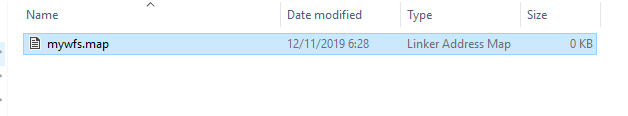
\includegraphics[width=4cm]{figures/Tugas4/1174077/16.png}
		\centering
		\caption{Membuat file baru}
    \end{figure}
  \item Modifikasi isinya menjadi sebagai berikut
  \hfill\break
    \begin{figure}[H]
		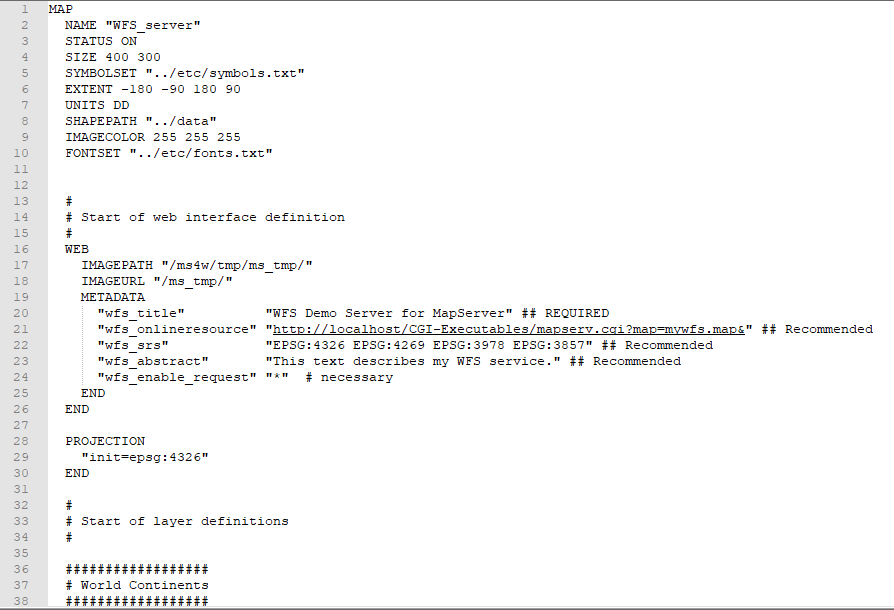
\includegraphics[width=4cm]{figures/Tugas4/1174077/17.png}
		\centering
		\caption{Isi mywfs.map 1}
    \end{figure}
  \item Kemudian Buka Browser dan Karena kalo diketik manual kepanjangan
  \item Nanti akan muncul tampilan XML
  \hfill\break
    \begin{figure}[H]
		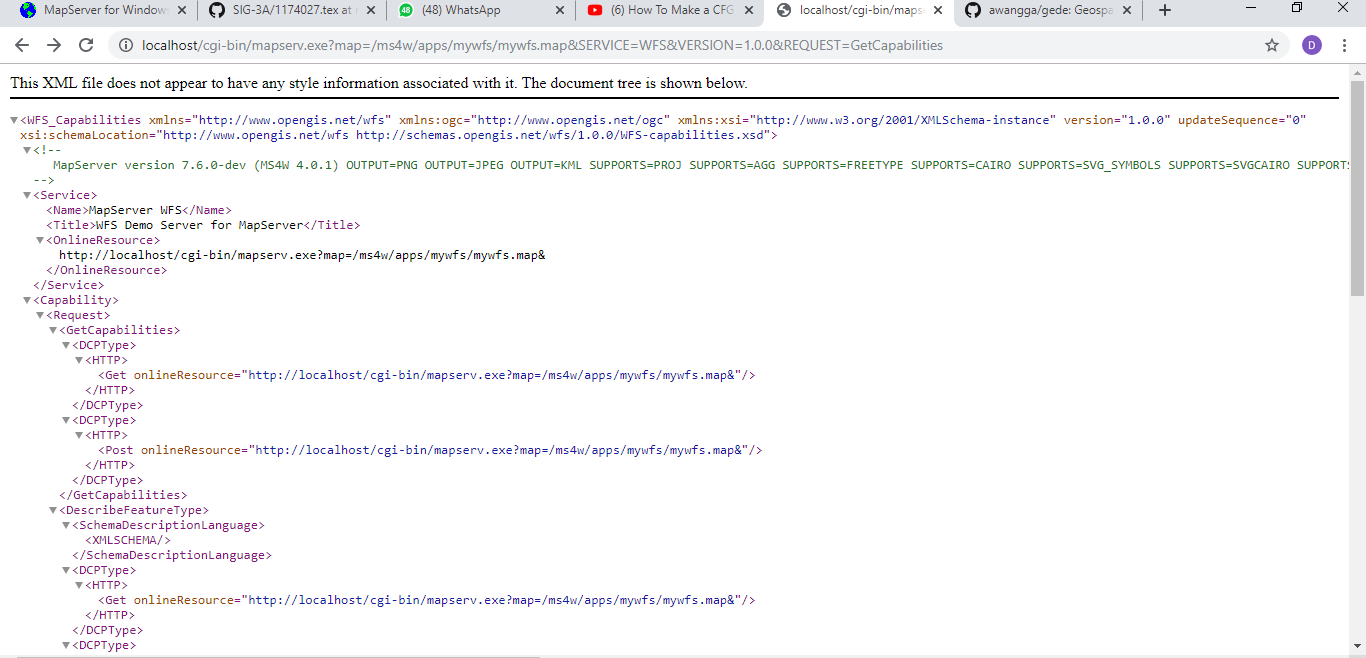
\includegraphics[width=4cm]{figures/Tugas4/1174077/18.png}
		\centering
		\caption{Tampilan Web}
    \end{figure}
  \item Kemudian Copy dan Buat file baru dengan nama sesuaikan dengan .shp nya dan extensinya .xml
  \item Simpan didalam folder bersama dengan shp filenya
  \hfill\break
  \begin{figure}[H]
  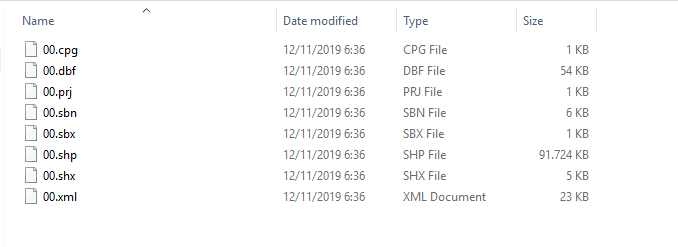
\includegraphics[width=4cm]{figures/Tugas4/1174077/19.png}
  \centering
  \caption{File shp dengan XML}
  \end{figure}
  \item Dan sekarang buka file .shp nya, dan lihat hasil nya
  \hfill\break
  \begin{figure}[H]
  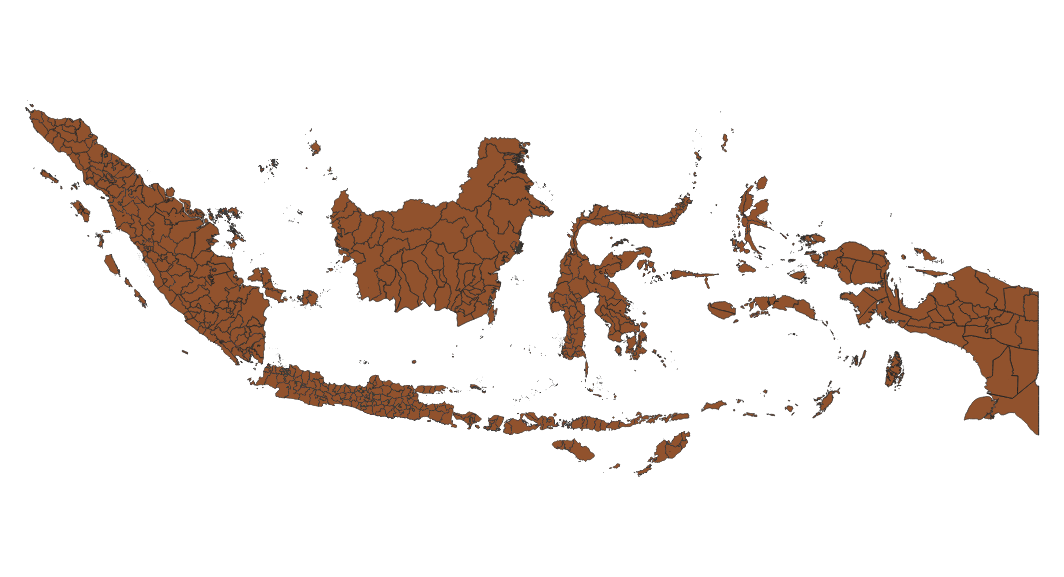
\includegraphics[width=4cm]{figures/Tugas4/1174077/map.png}
  \centering
  \caption{Hasil}
  \end{figure}
\end{enumerate}